\section{From double categories to bicategories}
\label{sec:1x1-to-bicat}

We are now equipped to lift structures on fibrant double categories to
their loose bicategories.  In this section we show that passage
from fibrant double categories to bicategories is given by a functor of a suitable sort.

As a point of notation, we write $\odot$ for the composition of
1-cells in a bicategory, since our bicategories are generally of the
form $\cH(\lD)$.  As advocated by Max Kelly, we say \textbf{functor}
to mean a morphism between bicategories that preserves composition up
to isomorphism; equivalent terms include \emph{weak 2-functor},
\emph{pseudofunctor}, and \emph{homomorphism}.

Recall that the assignment $\cH$ sends each double category $\lC$ to the loose bicategory  $\cH(\lD)$ of objects, 1-cells, and globular 2-morphisms of $\lD$.  Note that functors of double categories and bicategories compose strictly associatively; hence, we can talk about the 1-categories of double categories and bicategories, which we denote ${\bf Dbl}$ and ${\bf Bicat}$ respectively.

\begin{thm}\label{thm:1-func}
 If \lD\ is a double category, then $\cH(\lD)$ is a bicategory, and
  any functor $F\maps \lD\to\lE$ induces a functor $\cH(F)\maps
  \cH(\lD)\to\cH(\lE)$.  In this way $\cH$ defines a functor of
  1-categories $\mathbf{Dbl}\to \mathbf{Bicat}$.
\end{thm}
\begin{proof}
 The constraints of $F$ are all globular, hence give constraints for
  $\cH(F)$.  Functoriality is evident.
\end{proof}

% MS: This doesn't really make precise sense, and I'm not sure it's necessary.
%Note that this is a stronger condition than we need for our main result.
The action of \cH\ on transformations is less obvious. It
requires the presence of companions or conjoints, to lift the part of the data given by vertical morphisms to loose 1-cells. Before we discuss how this works, we briefly recall some definitions regarding transformations between functors of bicategories.

If $F,G\maps \cA\to\cB$ are functors between bicategories, then an
\textbf{oplax transformation} $\al\maps F\to G$ consists of 1-cells
$\al_A\maps FA\to GA$ and 2-cells
\[\vcenter{\xymatrix{ \ar[r]^{Ff}\ar[d]_{\al_A} \drtwocell\omit{\al_f} &  \ar[d]^{\al_B}\\
  \ar[r]_{Gf} & }}\]
such that for any 2-cell $\xymatrix{A \rtwocell^f_g{x} & B}$ in \cA,
\begin{equation}
  \label{eq:laxtransf-nat}
  \vcenter{\xymatrix@R=1pc@C=3pc{
      \rtwocell^{Ff}_{Fg}{Fx}\ar[dd]_{\al_A} 
      &  \ar[dd]^{\al_B}\\
      \drtwocell\omit{\al_g} & \\
      \ar[r]_{Gg} & }}\;=\;
  \vcenter{\xymatrix@R=1pc@C=3pc{
      \ar[r]^{Ff}\ar[dd]_{\al_A} \drtwocell\omit{\al_f} &
      \ar[dd]^{\al_B}\\ & \\
      \rtwocell^{Gf}_{Gg}{Gx} & }}
\end{equation}
and moreover for any $A$ and any $f,g$ in \cA,
\begin{equation}
  \vcenter{\xymatrix@R=5pc{
      \rtwocell^{1_{FA}}_{F(1_A)}{\iso} \ar[d]_{\al_A} \drtwocell\omit{\al_{1_A}} &  \ar[d]^{\al_A}\\
      \rtwocell^{G(1_A)}_{1_{GA}}{\iso} & }} \;=\;
  \vcenter{\xymatrix{ \ar[r]^{1_{FA}}\ar[d]_{\al_A} \drtwocell\omit{\iso}&  \ar[d]^{\al_A}\\
      \ar[r]_{1_{GA}} &
    }}
  \quad\text{and}\quad
  \vcenter{\xymatrix{
      \ar[r]|{Ff}\ar[d]_{\al_A} \drtwocell\omit{\al_f}
      \rruppertwocell^{F(gf)}{\iso}
      &
      \ar[r]|{Fg}\ar[d]|{\al_B} \drtwocell\omit{\al_g} &
      \ar[d]^{\al_C}\\
      \ar[r]|{Gf} \rrlowertwocell_{G(gf)}{\iso} & \ar[r]|{Gg} & }}
  \;=\;
  \vcenter{\xymatrix{ \ar[r]^{F(gf)}\ar[d]_{\al_A} \drtwocell\omit{\al_{gf}} &  \ar[d]^{\al_C}\\
      \ar[r]_{G(gf)} & }}\label{eq:laxtransf-ax}
\end{equation}
It is a \textbf{lax transformation} if the 2-cells $\al_f$ go the
other direction, and a \textbf{pseudo transformation} if they are
isomorphisms.

Inverses of morphisms in a category are unique when they exist, so for a morphism (and in particular a natural transformation) to be an isomorphism is only a property rather than a structure.
But since inverse equivalences of morphisms in a bicategory are unique only up to isomorphism, if we only know that a morphism has the property of being an equivalence, we have to make choices to find an inverse equivalence.
For many purposes (see e.g.~\cite{nick:tricats}) it is more useful to include a ``coherent'' inverse equivalence as specified data so that such choices are no longer necessary; in the case of transformations the result is called a pseudo natural adjoint equivalence.

Before defining these, we first consider a more general notion of ``conjunctonal transformation.''
By doctrinal adjunction~\cite{kelly:doc-adjn}, given collections of
1-cells $\al_A\maps FA\to GA$ and $\be_A\maps GA\to FA$ and
adjunctions $\al_A\adj \be_A$ in \cB, there is a bijection between
\begin{inparaenum}
\item collections of 2-cells $\al_f$ making $\al$ an oplax
  transformation and
\item collections of 2-cells $\be_f$ making $\be$ a lax
  transformation.
\end{inparaenum}
Two such transformations correspond under this bijection if and only if
\begin{equation}
  \vcenter{\xymatrix@-.5pc{F(f) \ar[r]^-{\eta \odot \mbox{\tiny id}_{F(f)}}
      \ar[d]_{\mbox{\tiny id}_{F(f)}\odot \eta} &
      \be_B\odot \al_B \odot F(f) \ar[d]^{\mbox{\tiny id}_{\be_B} \odot \al_f}\\
      F(f) \odot \be_A\odot \al_A\ar[r]_-{\be_f \odot \mbox{\tiny id}_{\al_A}} &
      \be_B\odot G(f) \odot \al_A}}
  \quad\text{and}\quad
  \vcenter{\xymatrix@-.5pc{\al_B\odot F(f)\odot \be_A
      \ar[r]^-{\mbox{\tiny id}_{\al_B}\odot \be_f}\ar[d]_{\al_f \odot \mbox{\tiny id}_{\be_A}}&
      \al_B \odot \be_B \odot G(f)\ar[d]^{\ep \odot \mbox{\tiny id}_{G(f)}}\\
      G(f)\odot \al_A\odot \be_A \ar[r]_-{\mbox{\tiny id}_{G(f)} \odot \ep} & G(f)}}\label{eq:conjtrans}
\end{equation}
commute.  If we have a pointwise adjunction between an oplax and a lax
transformation, whose 2-cell structures correspond under this
bijection, we call it a \textbf{conjunctional transformation}
$(\al\conj \be)\maps F\to G$.  (These are the conjoint pairs in a
double category whose loose arrows are lax transformations and
whose vertical arrows are oplax transformations.)

Of particular importance is the case when both $\al$ and \be\ are
pseudo natural and each adjunction $\al_A\adj \be_A$ is an adjoint
equivalence.  In this case we call $\al\conj \be$ a \textbf{pseudo
  natural adjoint equivalence}.  A pseudo natural adjoint equivalence
can equivalently be defined as an internal adjoint equivalence in the
bicategory $\cBicat(\cA,\cB)$ of functors, pseudo natural
transformations, and modifications $\cA\to\cB$. 

Recall also that if $\al,\al'\maps F\to G$ are oplax transformations,
a \textbf{modification} $\mu\maps \al\to\al'$ consists of 2-cells
$\mu_A\maps \al_A\to\al'_A$ such that
\begin{equation}
  \vcenter{\xymatrix@C=1pc@R=2.5pc{ \ar[rr]^{Ff}\dtwocell_{\al'_A}^{\al_A}{\mu_A}  &
      \drtwocell\omit{\al_f} &  \ar[d]^{\al_B}\\
      \ar[rr]_{Gf} && }} \quad=\quad
  \vcenter{\xymatrix@C=1pc@R=2.5pc{ \ar[rr]^{Ff}\ar[d]_{\al'_A} \drtwocell\omit{\al'_f} && 
      \dtwocell^{\al_B}_{\al'_B}{\mu_B}\\
      \ar[rr]_{Gf} && }}\label{eq:modif-ax}
\end{equation}
There is an evident notion of modification between lax transformations
as well.  Finally, given conjunctional transformations $\al\conj\be$
and $\al'\conj \be'$, there is a bijection between modifications
$\al\to\al'$ and $\be'\to\be$, where $\mu\maps \al\to\al'$ corresponds
to $\bar{\mu}\maps \be'\to\be$ with components $\bar{\mu}_A$ defined
by:
\[\vcenter{\xymatrix@-.5pc{
    && FA \ar@{=}[drr] \ddtwocell<5>^{\al_A}_{\al'_A}{\mu_A}\\
    GA \ar[urr]^{\be'_A} \ar@{=}[drr] & \Swarrow_\ep && \Swarrow_\eta & FA\\
    &&GA\ar[urr]_{\be_A}
  }}\]
The modifications $\bar{\mu}$ and \mu\ are called \textbf{mates}, and
are compatible with composition (see \cite{ks:r2cats}).  Thus, given
$\cA,\cB$ we can define a bicategory $\Conj(\cA,\cB)$, whose objects
are functors $\cA\to\cB$, whose 1-cells are conjunctional
transformations considered as pointing in the direction of their left
adjoints, and whose 2-cells are mate-pairs of modifications.

% Note that a 2-cell $\al$ in \cDbl\ is an isomorphism just when each
%$\al_A$, \emph{and} each $\al_M$, is invertible.

\begin{thm}\label{thm:h-locfr}
  If \lD\ is a double category and \lE\ is a fibrant double category
  with chosen companions and conjoints, we have a functor of bicategories
  \begin{align}
    \cDbl(\lD,\lE) &\too \Conj(\cH(\lD),\cH(\lE))\\
    F &\mapsto \cH(F)\\
    \al &\mapsto (\alhat\conj\alchk).
  \end{align}
  Moreover, if \al\ is an isomorphism, then $\alhat\conj\alchk$ is a
  pseudo natural adjoint equivalence.
\end{thm}

Note that we are here regarding the 1-category $\cDbl(\lD,\lE)$ as a
bicategory with only identity 2-cells.

\begin{proof}
  We denote the chosen companion and conjoint of $f$ in \lE\ by \fhat\
  and \fchk, as usual.  We define $\alhat$ as follows: its 1-cell
  components are $\alhat_A = \widehat{\al_A}$, and its 2-cell
  component $\alhat_f$ is the composite
  \begin{equation}
    \vcenter{\xymatrix@R=1.5pc@C=2.5pc{
        \ar[r]|-@{|}^{U_{FA}}\ar@{=}[d] \ar@{}[dr]|{\Downarrow \eta_{\hat{\alpha}_A}} &
        \ar[r]^{Ff}\ar[d]|{\al_A} \ar@{}[dr]|{\Downarrow \al_f} &
        \ar[r]|-@{|}^{\alhat_B}\ar[d]|{\al_B} \ar@{}[dr]|{\Downarrow \epsilon_{\hat{\alpha}_B}} &
        \ar@{=}[d]\\
        \ar[r]|-@{|}_{\alhat_A} &
        \ar[r]_{Gf} &
        \ar[r]|-@{|}_{U_{GB}} & 
      }}\label{eq:oplax-2cell}
%     \vcenter{\xymatrix@R=1.5pc@C=2.5pc{
%         \ar[r]|-@{|}^{Ff}\ar@{=}[d] \ar@{}[drrr]|{\iso} &
%         \ar[rr]|-@{|}^{\alhat_B} &&
%         \ar@{=}[d]\\
%         \ar[r]|-@{|}^{U_{FA}}\ar@{=}[d] \ar@{}[dr]|{\Downarrow} &
%         \ar[r]|{Ff}\ar[d]|{\al_A} \ar@{}[dr]|{\Downarrow \al_f} &
%         \ar[r]|-@{|}^{\alhat_B}\ar[d]|{\al_B} \ar@{}[dr]|{\Downarrow} &
%         \ar@{=}[d]\\
%         \ar[r]|-@{|}_{\alhat_A} \ar@{=}[d] \ar@{}[drrr]|\iso &
%         \ar[r]|{Gf} &
%         \ar[r]|-@{|}_{U_{GB}} & \ar@{=}[d]\\
%         \ar[r]|-@{|}_{\alhat_A} & \ar[rr]|-@{|}_{Gf} &&
%       }}\label{eq:oplax-2cell}
  \end{equation}
  Equations~\eqref{eq:laxtransf-nat} and~\eqref{eq:laxtransf-ax}
  follow directly from \autoref{thm:dbl-transf}.  The construction of
  $\alchk$ is dual, using conjoints, and \autoref{thm:compconj-adj}
  shows that $\alhat_A\adj \alchk_A$.  For the first equation
  in~\eqref{eq:conjtrans}, we have
  \begin{equation}
    \vcenter{\xymatrix@-.5pc{
        \ar[r]|-@{|}^{U_{FA}}\ar@{=}[d] \ar@{}[dr]|{=} &
        \ar[r]|-@{|}^{Ff}\ar@{=}[d] \ar@{}[dr]|{=} &
        \ar[r]|-@{|}^{U_{FB}}\ar@{=}[d] \ar@{}[dr]|{\Downarrow \eta_{\hat{\alpha}_B}} &
        \ar[r]|-@{|}^{U_{FB}}\ar[d]|{\al_B} \ar@{}[dr]|{\Downarrow \eta_{\check{\alpha}_B}} &
        \ar@{=}[d]\\
        \ar[r]|{U_{FA}}\ar@{=}[d] \ar@{}[dr]|{\Downarrow \eta_{\hat{\alpha}_A}} &
        \ar[r]|{Ff}\ar[d]|{\al_A} \ar@{}[dr]|{\Downarrow\al_f} &
        \ar[r]|{\alhat_B}\ar[d]|{\al_B} \ar@{}[dr]|{\Downarrow \epsilon_{\hat{\alpha}_B}} &
        \ar[r]|{\alchk_B}\ar@{=}[d] \ar@{}[dr]|{=} &
        \ar@{=}[d]\\
        \ar[r]|-@{|}_{\alhat_A} &
        \ar[r]|-@{|}_{Gf} &
        \ar[r]|-@{|}_{U_{GB}} &
        \ar[r]|-@{|}_{\alchk_B} &
      }}\;=\;
    \vcenter{\xymatrix@-.5pc{
        \ar[r]|-@{|}^{U_{FA}}\ar@{=}[d] \ar@{}[dr]|{\Downarrow \eta_{\hat{\alpha}_A}} &
        \ar[r]|-@{|}^{Ff}\ar[d]|{\al_A} \ar@{}[dr]|{\Downarrow \al_f} &
        \ar[r]|-@{|}^{U_{FB}}\ar[d]|{\al_B} \ar@{}[dr]|{\Downarrow \eta_{\check{\alpha}_B}} &
        \ar@{=}[d]\\
        \ar[r]|-@{|}_{\alhat_A} &
        \ar[r]|-@{|}_{Gf} &
        \ar[r]|-@{|}_{\alchk_B} &
      }}\;=\;
    \vcenter{\xymatrix@-.5pc{
        \ar[r]|-@{|}^{U_{FA}}\ar@{=}[d] \ar@{}[dr]|{\Downarrow \eta_{\hat{\alpha}_A}} &
        \ar[r]|-@{|}^{U_{FA}}\ar[d]|{\al_A} \ar@{}[dr]|{\Downarrow \eta_{\check{\alpha}_A}} &
        \ar[r]|-@{|}^{Ff}\ar@{=}[d] \ar@{}[dr]|{=} &
        \ar[r]|-@{|}^{U_{FB}}\ar@{=}[d] \ar@{}[dr]|{=} &
        \ar@{=}[d]\\
        \ar[r]|{\alhat_A}\ar@{=}[d] \ar@{}[dr]|{=} &
        \ar[r]|{\alchk_A}\ar@{=}[d] \ar@{}[dr]|{\Downarrow \epsilon_{\check{\alpha}_A}} &
        \ar[r]|{Ff}\ar[d]|{\al_A} \ar@{}[dr]|{\Downarrow\al_f} &
        \ar[r]|{U_{FB}}\ar[d]|{\al_B} \ar@{}[dr]|{\Downarrow \eta_{\check{\alpha}_B}} &
        \ar@{=}[d]\\
        \ar[r]|-@{|}_{\alhat_A} &
        \ar[r]|-@{|}_{U_{GA}} &
        \ar[r]|-@{|}_{Gf} &
        \ar[r]|-@{|}_{\alchk_B} &
        }},
  \end{equation}
  and the second is dual.  Thus $(\alhat\conj\alchk)$ is a
  conjunctional transformation.

  It is left to construct the constraints and check the axioms for functors of bicategories. Suppose we are given $\al\maps F\to G$ and $\be\maps G\to H$.  Then by
  \autoref{thm:comp-compose}, $\behat_A\odot\alhat_A$ is a companion
  of $\be_A\circ \al_A$, so we have a canonical isomorphism given by the icon
  \[\theta_{\widehat{\be\al}_A, \,\behat_A\odot\alhat_A}\maps
  \widehat{\be\al}_A \too[\iso] \behat_A\odot\alhat_A.
  \]
  Of course, we also have $\theta_{\widehat{1_A},U_A}\maps
  \widehat{1_A} \too[\iso] U_A$ by \autoref{thm:comp-unit}.  These
  constraints are automatically natural, since $\cDbl(\lD,\lE)$ has no
  nonidentity 2-cells.  The axiom for the composition constraint says
  that two constructed isomorphisms of the form
  \[\widehat{\gm\be\al}_A \too[\iso] (\gmhat_A \odot \behat_A)\odot \alhat_A\]
  are equal.  However, both $\widehat{\gm\be\al}_A$ and $(\gmhat_A
  \odot \behat_A)\odot \alhat_A$ are companions of $\gm_A\be_A\al_A$,
  and both of these isomorphisms are constructed from composites of $\theta$s;
  hence they are both equal to
  \[\theta_{\widehat{\gm\be\al}_A,\, (\gmhat_A \odot \behat_A)\odot
    \alhat_A}\] and thus equal to each other.  The same argument
  applies to the axioms for the unit constraint; thus we have a functor of bicategories.

  Finally, if $\al$ is an isomorphism, then in particular each $\al_A$
  is an isomorphism, so by \autoref{thm:compconj-adj} each
  $\alhat_A\adj \alchk_A$ is an adjoint equivalence.  But \al\ being
  an isomorphism also implies that each 2-cell
  \[\vcenter{\xymatrix@-.5pc{ \ar[r]|-@{|}^-{Ff} \ar[d]_{\al_A} \ar@{}[dr]|{\Downarrow\al_f} &  \ar[d]^{\al_B}\\
      \ar[r]|-@{|}_-{Gf} & }}\]
  is an isomorphism.  From its inverse we form the composite
  \[\vcenter{\xymatrix@R=1.5pc@C=3pc{
      \ar[r]|-@{|}^{\alhat_A}\ar@{=}[d] \ar@{}[dr]|{\Downarrow \eta_{\hat{\alpha}_A^{-1}}} &
      \ar[r]^{Gf}\ar[d]|{\al_A\inv} \ar@{}[dr]|{\Downarrow\al_f\inv} &
      \ar[r]|-@{|}^{U_{GB}}\ar[d]|{\al_B\inv} \ar@{}[dr]|{\Downarrow \epsilon_{\hat{\alpha}_B^{-1}}} &
      \ar@{=}[d]\\
      \ar[r]|-@{|}_{U_{FA}}&
      \ar[r]_{Ff} &
      \ar[r]|-@{|}_{\alhat_B} &
    }}\]
%   \[\vcenter{\xymatrix@R=1.5pc@C=3pc{
%       \ar[r]|-@{|}^{\alhat_A}\ar@{=}[d] \ar@{}[drrr]|{\iso} &
%       \ar[rr]|-@{|}^{Gf} &&
%       \ar@{=}[d]\\
%       \ar[r]|-@{|}^{\alhat_A}\ar@{=}[d] \ar@{}[dr]|{\Downarrow} &
%       \ar[r]|{Gf}\ar[d]|{\al_A\inv} \ar@{}[dr]|{\Downarrow\al_f\inv} &
%       \ar[r]|-@{|}^{U_{GB}}\ar[d]|{\al_B\inv} \ar@{}[dr]|{\Downarrow} &
%       \ar@{=}[d]\\
%       \ar[r]|-@{|}_{U_{FA}} \ar@{=}[d] \ar@{}[drrr]|\iso &
%       \ar[r]|{Ff} &
%       \ar[r]|-@{|}_{\alchk_A} & \ar@{=}[d]\\
%       \ar[r]|-@{|}_{Ff} &
%       \ar[rr]|-@{|}_{\alchk_A} &&
%     }}\]
  which we can then verify to be an inverse of~\eqref{eq:oplax-2cell}.
  Thus $\alhat$, and dually $\alchk$, is pseudo natural, and hence
  $\alhat\conj\alchk$ is a pseudo natural adjoint equivalence.
\end{proof}

We can also promote \autoref{thm:theta} to a functorial uniqueness.

\begin{lem}\label{thm:h-locfr-uniq}
  Let \lD\ be a double category and \lE\ a fibrant double category
  with two different sets of choices $\fhat,\fchk$ and $\fhat',\fchk'$
  of companions and conjoints for each vertical 1-morphism $f$, giving
  rise to two different functors
  \[\cH,\cH'\maps \cDbl(\lD,\lE)\too \Conj(\cH(\lD),\cH(\lE)).\]
  Then the isomorphisms $\theta$ from \autoref{thm:theta} fit together
  into a pseudo natural adjoint equivalence $\cH\eqv \cH'$ that is the
  identity on objects (an ``invertible icon'').
\end{lem}
\begin{proof}
  We must first show that for a given transformation $\al\maps F\to
  G\maps \lD\to\lE$ in \cDbl, the isomorphisms \th\ correspond to 2-cells $\alhat \iso \alhat'$ of $\Conj(\cH(\lD),\cH(\lE))$; that is, they form invertible
  modifications.
  Substituting~\eqref{eq:oplax-2cell} and the definition of \th\
  into~\eqref{eq:modif-ax}, this becomes the assertion that
  \begin{equation}
    \vcenter{\xymatrix@R=1.5pc@C=2pc{
        &
        \ar[r]|-@{|}^{U_{FA}}\ar@{=}[d] \ar@{}[dr]|{\Downarrow \eta_{\hat{\alpha}_A}} &
        \ar[r]^{Ff}\ar[d]|{\al_A} \ar@{}[dr]|{\Downarrow \al_f} &
        \ar[r]|-@{|}^{\alhat_B}\ar[d]|{\al_B} \ar@{}[dr]|{\Downarrow \epsilon_{\hat{\alpha}_B}} &
        \ar@{=}[d]\\
        \ar[r]|-@{|}^{U_{FA}} \ar@{=}[d] \ar@{}[dr]|{\Downarrow \eta_{\hat{\alpha}_A'}} &
        \ar[r]|{\alhat_A} \ar[d]|{\al_A} \ar@{}[dr]|{\Downarrow \epsilon_{\hat{\alpha}_A}}&
        \ar[r]_{Gf}  \ar@{=}[d] &
        \ar[r]|-@{|}_{U_{GB}} & \\
        \ar[r]|-@{|}_{\alhat_A'} & \ar[r]|-@{|}_{U_{GB}}&&
      }} \;=\;
    \vcenter{\xymatrix@R=1.5pc@C=2pc{
        && \ar@{=}[d] \ar[r]|-@{|}^{U_{FA}} \ar@{}[dr]|{\Downarrow \eta_{\hat{\alpha}_B'}} &
        \ar[d]|{\al_B} \ar[r]|-@{|}^{\alhat_B} \ar@{}[dr]|{\Downarrow \epsilon_{\hat{\alpha}_B}}
        &
        \ar@{=}[d] &\\
        \ar[r]|-@{|}^{U_{FA}}\ar@{=}[d] \ar@{}[dr]|{\Downarrow \eta_{\hat{\alpha}_A'}} &
        \ar[r]^{Ff}\ar[d]|{\al_A} \ar@{}[dr]|{\Downarrow \al_f} &
        \ar[r]|{\alhat_B'}\ar[d]|{\al_B} \ar@{}[dr]|{\Downarrow \epsilon_{\hat{\alpha}_B'}} &
        \ar@{=}[d] \ar[r]|-@{|}_{U_{GB}}&\\
        \ar[r]|-@{|}_{\alhat_A'} &
        \ar[r]_{Gf} &
        \ar[r]|-@{|}_{U_{GB}} & .
      }}
  \end{equation}
  This follows from two applications of~\eqref{eq:compeqn}, one for
  $\alhat_A$ and one for $\alhat_B'$.  (The mate of \th\ is, of
  course, uniquely determined.)  Now, to show that these form a pseudo
  natural adjoint equivalence, it remains only to check that they do,
  in fact, form a pseudo natural transformation which is the identity
  on objects, i.e.\ that~\eqref{eq:laxtransf-nat}
  and~\eqref{eq:laxtransf-ax} are satisfied.
  But~\eqref{eq:laxtransf-nat} is vacuous since $\cDbl(\lD,\lE)$ has
  no nonidentity 2-cells, and~\eqref{eq:laxtransf-ax} follows from uniqueness of $\theta$s,
  since all the constraints involved are also instances of \th.
\end{proof}



It seems that we should have a functor from fibrant double categories
to a tricategory of bicategories, functors, conjunctional
transformations, and modifications, but there is no tricategory
containing conjunctional transformations since the interchange law
only holds laxly.  Thus, we introduce the following definition.

\begin{defn}
  We will say that a transformation $\alpha$ in $\cDbl$ is \textbf{loosely strong} if $\hat\alpha$ is pseudonatural.
  % and \textbf{co-loosely strong} if $\check \alpha$ is pseudonatural.
\end{defn}

Let $\cDblf$
denote the sub-2-category of \cDbl\ containing the fibrant double
categories, all functors between them, and only loosely-strong transformations; we regard it as a tricategory with only identity 3-cells.
Let \cBicat\ denote the tricategory of
bicategories, functors, pseudo natural transformations, and
modifications.  We aim to define a functor of tricategories $\cH\maps \cDblf\to \cBicat$.

However, to avoid having to work with the full complicated definition of tricategory, we observe that both $\cDblf$ and $\cBicat$ are \textbf{iconic tricategories}, meaning that all of their associativity and unit constraints are given by \emph{icons}.
An icon is, morally speaking, an oplax transformation whose 1-cell components are all identities; but as noted by~\cite{lack:icons} this can be reexpressed without referring to these identity morphisms at all, yielding a definition that is easier to work with (because identity 1-cells in a bicategory are not strict).

\begin{defn}
Let $\cD, \cE$ be bicategories, and let $F,G: \cD \rightarrow \cE$ be pseudo functors. An {\bf icon} $\alpha: F \Rightarrow G$ is given by a family of 2-cells $\alpha_f : Ff \Rightarrow Gf$ indexed by the 1-cells of $\cD$, which are natural in $f$ and such that for all objects $A, B, C$ and 1-cells $A \xrightarrow{f} B \xrightarrow{g} C$ the following diagrams commute:
\[
\begin{tikzpicture}[xscale=1.5]
\node (tl) at (0,1) {$\id_{FA}$};
\node (tr) at (1,1) {$F \id_A$};
\node (bl) at (0,0) {$\id_{GA}$};
\node (br) at (1,0) {$G\id_A$};
\draw[doubletight] (tl) to node[above]{$\iso$} (tr);
\draw[doubletight] (bl) to node[below]{$\iso$} (br);
\draw[doubleeq] (tl) to (bl);
\draw[doubletight] (tr) to node[right]{$\alpha_{\id_A}$} (br);
\end{tikzpicture}\qquad
\begin{tikzpicture}[xscale=2]
\node (tl) at (0,1) {$Fg  Ff$};
\node (tr) at (1,1) {$F(gf)$};
\node (bl) at (0,0) {$Gg Gf$};
\node (br) at (1,0) {$G(gf)$};
\draw[doubletight] (tl) to node[above]{$\iso$} (tr);
\draw[doubletight] (bl) to node[below]{$\iso$} (br);
\draw[doubletight] (tl) to node[left]{$\alpha_g \alpha_f$}(bl);
\draw[doubletight] (tr) to node[right]{$\alpha_{gf}$} (br);
\end{tikzpicture}
\]
\end{defn}


As observed in~\cite{shulman:psalg}, an iconic tricategory can equivalently be viewed as a bicategory enriched over the bicategory \Icon\ of bicategories, functors, and icons (which has strict products).
That is, it is a structure \bS\ with objects, hom-bicategories $\bS(A,B)$, composition functors $\bS(B,C)\times \bS(A,B)$, identities $1_A \in \bS(A,A)$, and associativity and unitality \emph{icons} that satisfy the usual pentagon and triangle identities.
(There is no room for any higher coherence, since the data of an icon consists of 2-cells only.)
In particular, composition of 1-cells (objects of $\bS(A,B)$) is strictly associative, though the associativity for horizonatl composition of 2-cells is mediated by an icon.

Similarly, we have the notion of \textbf{iconic functor}, namely an \Icon-enriched functor of bicategories.
We can write this explicitly as follows.

\begin{defn}\label{def:Iconfunc}
Let ${\bf S,T}$ be \Icon-enriched bicategories. An \Icon-enriched functor $\cT: {\bf T} \rightarrow {\bf S}$ consists of the following data:
\begin{enumerate}
\item An assignment on objects that sends each object $A$ of ${\bf T}$ to an object $\cT A$ of ${\bf S}$.
\item For each two objects $A,B$, a functor (1-cell in \Icon) ${\bf T}(A,B) \rightarrow {\bf S}(\cT(A),\cT(B))$
\item For every triple of objects $A,B,C$ of ${\bf T}$, an invertible icon (2-cell in \Icon) 
\begin{align} 
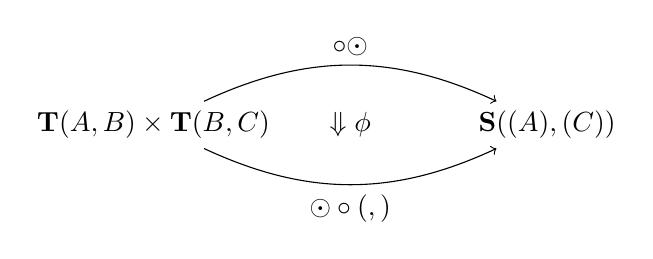
\begin{tikzpicture}
\node(1) at (0,0) {${\bf T}(A,B) \times {\bf T}(B,C)$};
\node(2) at (5,0) {${\bf S}(\cT(A),\cT(C))$};
\draw[->] (1) to[in=155, out=25] node[above]{$\cT \circ \odot$} (2); 
\draw[->] (1) to[in=-155, out=-25] node[below]{$\odot \circ (\cT,\cT)$} (2); 
\node at (2.5,0) {$\Downarrow \phi \iso$};
\end{tikzpicture}
\end{align}
where $\odot$ denotes loose composition.
\item For every object $A$ of {\bf T} an invertible icon
\begin{align}
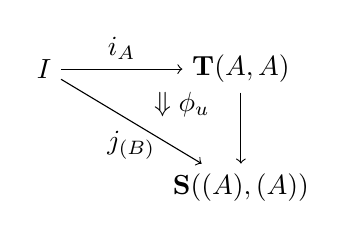
\begin{tikzpicture}[xscale=.5, yscale=.3]
\node(1) at (0,0) {$I$};
\node(2) at (5,0) {${\bf T}(A,A)$};
\node(3) at (5,-5) {${\bf S}(\cT(A),\cT(A))$};
\draw[->] (1) to node[above]{$i_{A}$} (2); 
\draw[->] (1) to node[below]{$j_{\cT(B)}$} (3);
\draw[->] (2) to node[right]{$\cT$} (3); 
\node at (3.5,-1.5) {$\Downarrow \phi_u \iso$};
\end{tikzpicture}
\end{align}
where $i$ and $j$ are the unitors of ${\bf S}$ and ${\bf T}$.
\item The usual coherence diagrams, Definition 10 of~\cite{nick:tricatsbook} commute.
\end{enumerate}
\end{defn}

\begin{thm}\label{thm:h-functor}
  There is an iconic functor $\cH\maps \cDblf\to \cBicat$.
\end{thm}
\begin{proof}
The first two requirements in \autoref{def:Iconfunc} are satisfied by Theorems \ref{thm:1-func} and \ref{thm:h-locfr} (ignoring the right adjoint parts of the conjunctional transformations).
The third requirement amounts to the existence of an invertible modification
%
\begin{equation}
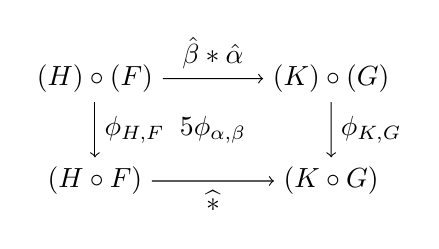
\begin{tikzpicture}[xscale=0.75, yscale=1.3]
\node (tl) at (0,2) {${\cH}(H) \circ {\cH}(F)$};
\node (bl) at (0,1) {${\cH}(H \circ F)$};
\node (tr) at (4,2) {${\cH}(K) \circ {\cH}(G)$};
\node (br) at (4,1) {${\cH}(K \circ G)$};
\draw[->] (tl) to node [above] {$\hat{\beta} * \hat{\alpha}$} (tr);
\draw[->] (tr) to node [right] {$\phi_{K,G}$} (br);
\draw[->] (tl) to node [right] {$\phi_{H,F}$} (bl);
\draw[->] (bl) to node [below] {$\widehat{\be*\al}$} (br);
\node at (2,1.5) {$\Arrow{5} \phi_{\alpha,\beta} $};
\end{tikzpicture}
\end{equation}
%
for every pair of transformations between fibrant double categories
  \[\vcenter{\xymatrix{\lC \rtwocell^F_G{\al} & \lD \rtwocell^H_K{\be}
      & \lE}}\]
satisfying the naturality and composition constraints~\eqref{eq:laxtransf-ax} and~\eqref{thm:1-func}.

However, since composition of
  1-cells in $\cDblf$ and \cBicat\ is strictly associative and
  unital, and \cH\ strictly preserves this composition (Theorem \ref{thm:1-func}),
  the composition constraints $\phi_{H,F}$ and $\phi_{K,G}$ are identities. Consequently, $\phi$ is merely  a modificaton $\phi\maps \behat * \alhat \iso \widehat{\be*\al}$ such that 
%
 \begin{equation}
        \vcenter{\xymatrix@-.5pc{
        1_{{\cH}H \circ {\cH}F} \ar[r]\ar[d]_{=} &
        \hat{1}_{K}*\hat{1}_{H}\ar[d]^{\phi}\\
        1_{{\cH}(H \circ F)}\ar[r] &
        \widehat{1_{K} *1_{H}}}} \quad\text{and}\quad       
    \vcenter{\xymatrix@-.5pc{
        \widehat{\gm\al}*\widehat{\de\be} \ar[r]\ar[d]_\phi &
        (\gmhat*\dehat)\odot(\alhat*\behat)\ar[d]^{\phi \odot \phi}\\
        \widehat{\gm\al*\de\be}\ar[r] &
        (\widehat{\gm*\de})\odot(\widehat{\al*\be})}}
  \end{equation}
commute. (Here we are writing $*$ for the `Godement product' of 2-cells in $\cDbl$ and $\cBicat$.)    
Note that condition~\eqref{eq:laxtransf-nat} is satisfied because $\cDblf$ has no nonidentity 3-cells.
  
  Now by Lemmas \ref{thm:comp-compose} and
  \ref{thm:comp-func}, $(\behat *\alhat)_A = \behat_{GA} \circ
  H(\alhat_A)$ is a companion of $(\be*\al)_A = \be_{GA} \circ
  H(\al_A)$.  Therefore, we take the component $(\phi_{\alpha,\beta})_A$ to be
  \[\theta_{\behat_{GA} \circ H(\alhat_A),\, \widehat{\be*\al}_A}.\]
  The equations above are satisfied by uniqueness of $\theta$-isomorphisms.
   Equation~\eqref{eq:modif-ax}, saying that these form a modification,
  becomes the equality of two large composites of 2-cells in \lD,
  which as usual follows from~\eqref{eq:compeqn}. The equations above are satisfied by uniqueness of $\theta$-isomorphisms.

The icon  $\phi_u$ is simply the identity, since $\cH$ is strictly unital.
    %Finally, the required
  %modifications merely amount to the \emph{assertions} that
  %\[\vcenter{\xymatrix@-.5pc{\gmhat*\behat*\alhat \ar[r]^\chi\ar[d]_\chi &
   %   \widehat{\gm*\be}*\alhat \ar[d]^\chi\\
   %   \gmhat*\widehat{\be*\al}\ar[r]_\chi & \widehat{\gm*\be*\al}}},\qquad
  %\vcenter{\xymatrix@-.5pc{ \alhat \ar[r]^-\iota \ar@{=}[dr] &
   %   \widehat{1_F}*\alhat \ar[d]^\chi \\ & \alhat }}, \;\text{and}\qquad
  %\vcenter{\xymatrix@-.5pc{ \alhat \ar[r]^-\iota \ar@{=}[dr] &
   %   \alhat*\widehat{1_F} \ar[d]^\chi \\ & \alhat }}\]
  %commute; again this follows from \autoref{thm:theta-compose-vert}.
\end{proof}

Our goal is to enhance this functor to act on ``monoidal objects''.
It is well-known that ``monoidal functors preserve monoid objects'', so our approach will be to categorify this: we will show that $\cH$ is monoidal, in an appropriate sense, and that monoidal functors of this sort preserve monoidal objects of the appropriate sort.

In fact, the monoidality of $\cH$ is easy to describe, because the monoidal structures of $\cDblf$ and $\cBicat$ are cartesian and very strict.
In general, if $\mathcal{V}$ is a monoidal 2-category with strict 2-categorical finite products (such as \Icon), we say that a $\mathcal{V}$-enriched bicategory ${\bf B}$ has \textbf{finite products} when for each two objects $C,D \in {\bf B}$ there is an object $C\times D$ with projections $C\times D\to C$ and $C\times D\to D$ (i.e.\ morphisms $I\to \mathbf{B}(C\times D,C)$ and $I\to \mathbf{B}(C\times D,D)$ in \cV) inducing an \emph{isomorphism} in $\mathcal{V}$ (not merely an equivalence):
%
\begin{align}
{\bf B}(A, C \times D) \xrightarrow{\cong} {\bf B}(A,C) \times {\bf B}(A,D)
\end{align}
and similarly there is a strict terminal object $\ast$ such that $\bB(A,\ast)$ is strictly terminal in \cV\ for all $A$.
This holds for \cBicat\ and \cDblf, because cartesian products of bicategories and double categories are simply componentwise, and all the morphisms in \cBicat\ and \cDblf\ (no matter how weak) are defined in terms of data in their targets.

Similarly, we say that a functor $F$ of \cV-enriched bicategories \textbf{preserves products} if it takes the terminal object to a terminal object and pairs of product projections $A \leftarrow A\times B \to B$ to pairs of product projections (in the above strict sense).

\begin{thm}
The iconic functor $\cH: \cDblf \rightarrow \cBicat$ preserves products.
\end{thm}
\begin{proof}
Since $\cH$ merely forgets a part of the double categories and double functors, we have simple equalities
$\cH(\mathbb{D} \times \mathbb{E}) = \cH(\mathbb{D}) \times \cH(\mathbb{E})$, and the product projections are likewise preserved.
The case of the terminal object is likewise easy.
\end{proof}

We end this section with one final lemma.

\begin{lem}\label{thm:theta-nat}
  Suppose $F,G\maps \lD\to\lE$ are functors of double categories, $\al\maps F\to G$ is a
  transformation, and that $f\maps A\to B$ has a companion \fhat\ in
  \lD.  Then the oplax comparison 2-cell for \alhat:
  \[\vcenter{\xymatrix{
      \ar[r]^{F(\fhat)}\ar[d]_{\alhat_A} \drtwocell\omit{\;\alhat_{\fhat}}&  \ar[d]^{\alhat_B}\\
      \ar[r]_{G(\fhat)} & }}\]
  is equal to $\theta_{\alhat_B\odot F(\fhat),\, G(\fhat) \odot
    \alhat_A}$ (and in particular is an isomorphism).
\end{lem}
\begin{proof}
  By definition $\alhat_A$ and $\alhat_B$ are companions of $\al_A$
  and $\al_B$, respectively, and by \autoref{thm:comp-func} $F(\fhat)$
  and $G(\fhat)$ are companions of $F(f)$ and $G(f)$, respectively.
  Thus, by \autoref{thm:comp-compose} the domain and codomain of
  $\alhat_{\fhat}$ are both companions of $G(f) \circ \al_A = \al_B
  \circ F(f)$, so at least the asserted $\theta$ isomorphism exists.
  Now, by taking the definition~\eqref{eq:oplax-2cell} of
  $\alhat_{\fhat}$ and substituting it for $\theta$
  in~\eqref{eq:comp-iso}, using the axioms for companions and the
  naturality of $\al$ on 2-morphisms, we see that $\alhat_{\fhat}$
  satisfies~\eqref{eq:comp-iso} and hence must be equal to $\theta$.
\end{proof}



% Local Variables:
% TeX-master: "smbicat"
% End:
